\documentclass[a4paper,11pt,final]{article}
% Pour une impression recto verso, utilisez plutôt ce documentclass :
%\documentclass[a4paper,11pt,twoside,final]{article}

\usepackage[english,francais]{babel}
\usepackage[utf8]{inputenc}
\usepackage[T1]{fontenc}
\usepackage[pdftex]{graphicx}
\usepackage{tikz}
\usepackage{setspace}
\usepackage{hyperref}
\usepackage[toc]{glossaries}
\usepackage[french]{varioref}
\usepackage{enumitem}

\makeglossaries

\newlist{arrowlist}{itemize}{1}
\setlist[arrowlist]{label=$\rightarrow$}

\newcommand{\reporttitle}{État de l'art des systèmes de gestion des comptes à privilèges}     % Titre
\newcommand{\reportauthor}{Alexandre \textsc{Kervadec}} % Auteur
\newcommand{\reportsubject}{Mémoire de stage de fin d'études} % Sujet
\newcommand{\HRule}{\rule{\linewidth}{0.5mm}}
\setlength{\parskip}{1ex} % Espace entre les paragraphes

\hypersetup{
    pdftitle={\reporttitle},%
    pdfauthor={\reportauthor},%
    pdfsubject={\reportsubject},%
    pdfkeywords={rapport} {IAM} {PAM} {synetis} {bordeaux} {rennes} {universite} {stage}
}

\begin{document}
  % Inspiré de http://en.wikibooks.org/wiki/LaTeX/Title_Creation

\begin{titlepage}

\begin{center}

\begin{minipage}[t]{0.48\textwidth}
  \begin{flushleft}
    
\includegraphics [width=60mm]{images/logo-univ.jpg} \\[0.5cm]
  \end{flushleft}
\end{minipage}
\begin{minipage}[t]{0.48\textwidth}
  \begin{flushright}
    
\includegraphics [width=30mm]{images/mini_logo_synetis.png} \\[0.5cm]
  \end{flushright}
\end{minipage} \\[1.5cm]

\textsc{\Large \reportsubject}\\[0.5cm]
\HRule \\[0.4cm]
{\huge \bfseries \reporttitle}\\[0.4cm]
\HRule \\[1.5cm]

\begin{minipage}[t]{0.3\textwidth}
  \begin{flushleft} \large
    \emph{Auteur :}\\
    \reportauthor
  \end{flushleft}
\end{minipage}
\begin{minipage}[t]{0.6\textwidth}
  \begin{flushright} \large
    \emph{Responsables :} \\
    M. Philippe \textsc{Rolland} \\
    M. Damien \textsc{Seiler} \\
    M. Mathieu \textsc{Raffinot}
  \end{flushright}
\end{minipage}

\vfill

{\large 2016}

\end{center}

\end{titlepage}

  \cleardoublepage % Dans le cas du recto verso, ajoute une page blanche si besoin
  \section*{Remerciements}
\addcontentsline{toc}{section}{Remerciements}

Je tiens tout particulièrement à remercier mes accompagnateurs chez \textsc{Synetis} : Damien Seiler et Philippe Rolland, qui m'ont aidé quotidiennement durant ce stage. Je remercie aussi tous les consultants de chez \textsc{Synetis}, qui ont, à des moments ponctuels, su m'enrichir de leur expertise. Il me semble aussi important de remercier Lionel Clément qui m'a suivi et aidé pour ma recherche de stage, lorsque j'avais un retard conséquent par rapport aux dates prédéfinies.
  \cleardoublepage
  \tableofcontents % Table des matières
  \sloppy          % Justification moins stricte : des mots ne dépasseront pas des paragraphes
  \cleardoublepage
  \listoffigures
  \addcontentsline{toc}{section}{Liste des figures}
  \cleardoublepage
  % \newglossaryentry{credential}
{
	name=credential,
	description={est le terme représentant les informations de connexion, comme par exemple un couple login/mot de passe ou une carte à puce}
}
\newglossaryentry{pam}
{
	name=PAM,
	description={Privileged Account Management : gestion des comptes à privilèges}
}
  \newglossaryentry{credential}{name=credential, description={est le terme représentant les informations de connexion, comme par exemple un couple login/mot de passe ou une carte à puce}}
  \newglossaryentry{pam}{name=PAM, description={Privileged Account Management : gestion des comptes à privilèges}}
  \newglossaryentry{bastion}{name=bastion, description={moteur de gestion des connexions aux ressources de la solution de PAM}}
  \newglossaryentry{stratch}{name={from stratch}, description={démarrer un projet depuis rien, à partir de zéro}}
  \printglossaries
  \cleardoublepage
  \section*{Introduction} % Pas de numérotation
\label{intro}
\addcontentsline{toc}{section}{Introduction} % Ajout dans la table des matières

%-> Environnement professionnel et l'entreprise. <-
%
%-> Objectifs du travail personnel et moyens mis en oeuvre pour les atteindre <-
%
%-> Présentation claire du plan adopté poru la suite du corps du mémoire <-
%
%Pas plus de 2 pages.
Le choix de mon entreprise de stage s'est orientée vers \textsc{Synetis}, qui est une porte ouverte vers le monde de la sécurité, dans lequel je souhaite m'orienter malgré ma formation qui n'est pas spécialisée dans ce domaine.\\
\textsc{Synetis} est une PME\footnote{Petite à Moyenne Entreprise} à taille humaine basée dans le centre de Paris. Une agence a été ouverte à Rennes en 2012 lors du recrutement de spécialistes en gestion des identités sur cette zone. Cette agence de Rennes compte 6 consultants et 2 managers (dont le chef d'agence). L'ambiance est très conviviale, tout le monde se connaît, des évènements de cohésion sont régulièrement organisés (afterwork, repas en groupe le vendredi midi). De même, une réunion trimestrielle est organisée sur le siège de Paris, qui regroupe tout le personnel de \textsc{Synetis}, afin de faire un bilan des projets, de rencontrer les nouveaux arrivants, et de partager les nouveaux objectifs visés par l'entreprise.\\
Le travail est réparti par équipe sur les différents projets en cours, chaque consultant pouvant travailler sur plusieurs projets en même temps. On peut distinguer deux types de projet : les gros projets s'étalant sur de longues périodes (plus de six mois) et les projets courts durant au maximum quatre mois. L'entreprise est spécialisée dans la gestion d'identité pour les grands groupes (conseils régionaux, grandes entreprises nationales et internationales), mais commence à développer une branche de pentest (test d'intrusion sur différentes structures, pour de plus amples informations, le guide de Rafay Baloch \cite{rba} est très complet).\\
J'étais intégré comme tous les autres consultants, avec un tuteur travaillant sur des projets correspondants au sujet de mon stage qui me guidait au travers de mes recherches et développements.\\
Ce stage concerne les systèmes de gestion de comptes à privilèges, qui sont les comptes avec des droits élevés, comme ceux des compte \textsc{root} des systèmes d'exploitation Linux/UNIX et \textsc{Administrateur} sur Windows. Durant ce stage, il était question de comprendre ne profondeur les enjeux de la gestion de comptes à privilèges, les moyens existant pour établir cette gestion pour pouvoir mieux comparer l'ensemble des solutions disponibles sur le marché. Cette comparaison a permis de considérer 2 solutions à mettre en œuvre sur un environnement virtuel pour comprendre ces systèmes dans les moindres détails, et en faire une comparaison encore plus poussée. Toutes les informations récoltées nous auront finalement permis de comprendre comment les solutions répondent à la problématique de la gestion des comptes à privilèges, et de déterminer quelles solutions répondent le mieux à cette problématique, afin de pouvoir proposer de l'intégration avec de futurs clients.

Le plan adopté pour la suite de ce mémoire consiste en une première section décrivant la problématique à résoudre, et les origines de cette problématique. Une deuxième section expliquera les moyens et les méthodes mises en œuvre pour répondre à cette problématique et enfin une dernière partie expliquera les résultats obtenus.
  \cleardoublepage
  %\section{Section}
%
%\subsection{Sous section}
%
%\subsubsection{Sous sous section}
%
%\paragraph{Paragraphe}
%
%Pas plus bas dans la hiérarchie. Minimum 2 éléments par division hiérarchique.
%
%Equilibrer la taille de chaque chapitre (à l'exception de l'introduction et de la conclusion).
%
%Exemple de développement :
%- Problématique
%- Matériels et méthodes
%- Résultats et discussion

%\begin{figure}[!ht]
%    \center
%    
\includegraphics[width=0.5\textwidth]{./images/logo-univ.jpg}
%    \caption{logo université, échelle 50\% de la page}
%\end{figure}
\section{Problématique : comment pallier le manque de contrôle des comptes privilégiés}

L'objectif général est de résoudre le problème de manque de contrôle et de monitoring des comptes à privilèges. Afin de parvenir à ce résultat, plusieurs solutions ont été développées par des éditeurs, le but final de ce projet étant de déterminer quelle est, ou quelles sont, la ou les meilleures solutions permettant de résoudre ce problème.\\
Pour répondre à cette problématique, nous allons d'abord expliquer plus en détails ce qu'est un compte à privilèges, puis nous intéresser aux raisons pour lesquelles ces comptes sont des points clefs de la sécurité des systèmes d'information. Ensuite, nous allons expliquer un fonctionnement global et commun aux solutions du marché puis mettre en avant les limitations que peuvent avoir ces solutions de PAM.

\subsection{Contexte}

La gestion de comptes à privilèges (PAM\footnote{Privileged Access Management}) est une sous-section de la gestion d’identité et d’accès (IAM\footnote{Identity and Access Management}). L’IAM est un large champ de contrôle d’accès qui se veut critique dans le domaine des technologies de l’information.\\
Il existe bien sûr une multitude de connexions spécifiques entre les utilisateurs et les dépendances technologiques. La PAM n’est que l’une d’entre elles.\\
La PAM est apparue au début des années 2000 à cause de l’impossibilité des solutions d’IAM de contrôler, gérer et faire des rapports sur les accès aux serveurs, aux bases de données, aux équipements réseau et tout autre application critique au sein d’une organisation. Cette solution entraîne une gestion d’un petit nombre d’utilisateurs, mais d’un grand nombre de dépendances technologiques ayant une importance clef dans le fonctionnement des infrastructures.\\
La fonctionnalité principale d’une solution de gestion d’identité privilégiée gravite autour de la sécurisation de l’accès aux ressources critiques par les administrateurs IT.\\
Plus précisément, des privilèges spécifiques peuvent être délivrés à des comptes d’utilisateur. Ces privilèges sont dépendants des systèmes et des applications impliqués, mais ils peuvent inclure la capacité à écrire des données, créer des comptes, exécuter une mission, pour ne citer que quelques exemples. En plus de contrôler l’accès avec un grand niveau de finesse, beaucoup de solutions fournissent aussi un package d’actions disponibles lors de l’utilisation d’un compte privilégié. Dans le but d’assurer la sécurité de ces comptes, les solutions exploitent un large éventail de mécanismes, comme par exemple, l’utilisation de clefs SSH, la rotation de mot de passe et l’ajout de multiples authentifications (authentification multi-facteur).\\
La gestion d’identités privilégiées est devenue de plus en plus importante, notamment avec la croissance des requis de sécurité et des règles de conformité (l’ISO 27001 qui est une norme de sécurité international sur la protection des actifs informationnels par exemple). Il est aussi important de noter que de nombreux exploits\footnote{Element permettant d'exploiter une faille de sécurité} compromettant des données sont liés à la compromission d’accréditations privilégiées. Avec la recrudescence des tentatives de hack et les contrecoups économiques de plus en plus conséquents, les entreprises commencent à apporter de plus en plus d’intérêt à la gestion et au contrôle des comptes à privilèges. En effet, les tentatives de piratage sont de plus en plus variées : du social engineering, au vol de ces accréditations par une brèche dans la sécurité en passant par des \textit{brute force} de mot de passe n’ayant pas une complexité suffisante\footnote{L'utilisation de mots de passe faibles tels que \texttt{password}, \texttt{admin}, \texttt{1234}, \texttt{azerty1234} ou \texttt{Abcd1234} reste encore très fréquente. Pour trouver ces mots de passe faibles, la technique la plus employée est le brute force avec un dictionnaire de mots de passe}.\\

\subsection{Un point clef de la sécurité des systèmes d'information}

\paragraph{Une cible de choix pour les pirates}
Un compte privilégié est un compte utilisé par les administrateurs système et réseau, ainsi que par les équipes de sécurité pour accéder aux ressources réseau comme les serveurs, les pare-feux, les switches, les routeurs, les ordinateurs, les applications ou les base de données avec des droits élevés. Ces comptes sont nécessaire à la maintenance d'une infrastructure, tout comme aux interventions de réparation, de diagnostique ou gestion de situations de crise\footnote{Attaque sur un serveur par exemple}. Dans de grands groupes, il peut y avoir un grand nombre de ces comptes, de l'ordre de la centaine voir du millier d'entités, réparti sur plusieurs sites.\\
Ces comptes peuvent aussi être des comptes d'application communicant avec d'autres applications\footnote{A2A : Application To Application, littéralement d'application à application}, comme par exemple un serveur faisant une sauvegarde régulière sur un autre serveur de récupération.\\
Tous ces comptes ne sont pas surveillés par les traditionnels gestionnaires d'identités, seul un mot de passe permet d'y accéder. De plus ces comptes sont très souvent des comptes partagés entre plusieurs administrateurs pour une question de facilité de gestion.\\
Ainsi, une personne mal intentionnée réussissant à voler les accès d'un tel compte verrait son pouvoir de destruction, voir de vol d'information sans limites, ce qui en fait une cible privilégiée par les pirates informatiques.

\paragraph{Un manque de visibilité d'actions} Comme abordé en introduction, il existe un grand manque de visibilité sur les actions des comptes à privilèges. En effet, ces comptes aux droits élevés, ne sont ni tracés, ni surveillés. Ceci peut avoir plusieurs mauvaises incidences, certaines intentionnelles et malveillantes, d'autre involontaires mais tout de même paralysantes.\\
On peut classer ces incidences en deux catégories, l'une relevant d'une erreur accidentelle, et l'autre d'une volonté de nuire à une organisation :
\begin{itemize}
	\item Erreur accidentelle :
	\begin{arrowlist}
		\item Erreur de configuration, difficile à retrouver à cause du manque de supervision
	\end{arrowlist}
	\item Volonté de nuire :
	\begin{arrowlist}
		\item Sabotage d'une configuration, menant à un déni de service
		\item Vol d'informations sensibles
	\end{arrowlist}
\end{itemize}

Ce manque de  visibilité crée aussi un point noir dans un audit de sécurité : il n'y a aucune détection de faille de sécurité concernant ces comptes.

\subsection{Objectifs d'un système de PAM}

D'après les points précédents, on peut en déduire les spécificités que nous voudrions améliorer vis-à-vis des comptes à privilèges :
\begin{itemize}
	\item Centraliser l’accès aux données de l’entreprise
 	\item Sécuriser les comptes à privilèges (duo identifiants et mot de passse)
 	\item Gérer de manière forte des mots de passe et établir une politique d’authentification forte
	\item Journaliser et superviser les activités des comptes à privilèges
\end{itemize}

\subsection{Fonctionnement d'un système de gestion de comptes à privilèges}

\paragraph{Cas général}
Le principe commun à toutes les solutions des éditeurs est la présence d'une identification sur un serveur central. On peut considérer 2 groupes : les comptes à privilèges et les ressources à protéger. Entre ces 2 entités vient s'intercaler le serveur d'identification, qui fait la passerelle entre les comptes et les ressources.\\
L'identification d'un utilisateur sur un compte à privilèges se fait sur le serveur central, et l'identification de ce compte à privilèges sur une ressource protégée est déléguée au serveur central. Ainsi, les utilisateurs n'ont plus à gérer et connaître les mots de de passe d'accès au ressources protégées; c'est le serveur central qui détient tous les secrets\footnote{Les logins et mot de passe, aussi appelés \og credrentials \fg{} en anglais.}.\\
Le serveur central a à sa charge de protéger les mots de passe dans un coffre-fort et de les renouveler régulièrement.

\begin{figure}[!ht]
    \center
    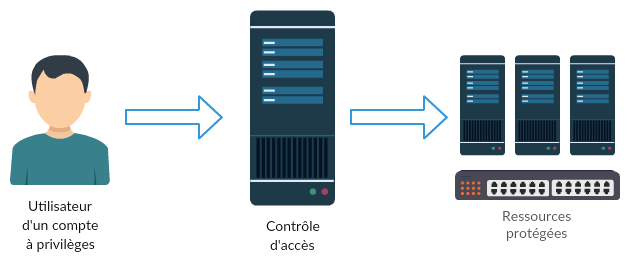
\includegraphics[width=\textwidth]{./images/Schema_ultra_light_PAM.png}
    \caption{Fonctionnement général d'un système de PAM}
\end{figure}

\paragraph{Deux types d'architecture}
Malgré le principe de fonctionnement identique pour quasiment toutes les solutions de PAM, il existe cependant des différences au niveau de l'architecture de ces dernières solutions, on distingue 2 grandes familles :
\begin{itemize}
	\item Architecture proxy\footnote{Toutes les communications transitent par un point de contrôle.} : les ressources et les comptes d'utilisateurs sont séparés physiquement (ou logiquement\footnote{Redirection des paquet  par port.}), le serveur central gère tout seul les accès aux applications
	\item Architecture avec agents : les accès aux ressources et la supervision sont gérés par des agents sur les ressources cibles (application installée sur la ressource)
\end{itemize}
Nous pouvons rapidement nous rendre compte qu'une architecture avec des agents est beaucoup plus intrusive et longue ou difficile à mettre en place qu'une architecture en proxy, où seul l'adressage est à modifier.

\subsection{Les limitations des solutions PAM}

\paragraph{Le facteur humain} Il faut noter que même avec un système de PAM éprouvé et efficace, nous ne pouvons pas mettre de côté le risque le plus exploitable dans le domaine de la sécurité qu'est le facteur humain. En effet, il est souvent plus facile de tromper un élément du personnel pour une compromission de données. Il sera donc important lors d'un déploiement d'une solution de PAM, d'éduquer le personnel de l'organisation concernée, afin que ces derniers mettent correctement en œuvre les règles de base de la sécurité informatique comme par exemple :
\begin{itemize}
	\item Totalement prohiber \og l'effet \textit{post-it} \fg{} : notation de mot de passe sur un \textit{post-it} collé sur l'écran
	\item  
\end{itemize}

\paragraph{La détection de comportements anormaux}
Très peu de solutions de PAM proposent un système de détection de comportements anormaux, comme par exemple un conseiller commercial qui aurait accès aux informations des comptes client, qui abuserait de ce droit.\\
En effet, même avec une restriction des droits, une supervision et journalisation des activités, une solution de PAM n'est pas une intelligence artificielle qui peut détecter des comportements suspect. Cependant, il est toujours possible de détecter des comportements prédéfinis avec des successions de commandes qui lèveraient une alerte.

%L’objectif est de mettre en place un système de contrôle des risques liés aux comptes à privilèges, donc tout d’abord avoir un socle central d’accès. Ce socle doit constituer l’élément central du système d'information par lequel circulent tous les flux venant des utilisateurs vers les données de l’entreprise. Ainsi, ce socle gère tous les accès aux ressources protégées, et les utilisateurs n’ont plus à connaître les mots de passe des ressources, mais juste leur mot de passe personnel pour se connecter au socle principal.\\
%Le choix d’une solution doit prendre en compte l’environnement technique, les habitudes des administrateurs et les logiciels utilisés par l’entreprise.\\
%Afin de parvenir à un système sûr et performant, nous pouvons dégager les objectifs suivants :
%\begin{itemize}
%	\item Centraliser l’accès aux données de l’entreprise.
%	\item Sécuriser les comptes à privilèges.
%	\item Gérer de manière forte des mots de passe et établir une politique d’authentification forte.
%	\item Journaliser les activités des comptes à privilèges.
%	\item Automatiser les processus pour améliorer la productivité tout en renforçant la sécurité.
%\end{itemize}
  \cleardoublepage
  \section{Méthodes et moyens mis en œuvre}
\label{sec:meth_moy}

Comme le titre l'indique, nous allons expliquer les méthodes et les moyens utilisés pour répondre à la problématique posée. Cette section sera séparée en 3 sous-sections : la première décrivant mon cheminement en matière de gestion de projet, la deuxième traitant de la phase de recherche d'informations, avec ses problèmes rencontrés et solutions trouvée, puis une troisième partie décrivant le travail effectué pendant la phase de test des deux produits sur un environnement de test, ainsi que toutes les différentes technologies utilisées.

\subsection{Gestion de projet}
\label{subsec:gestion}

La première chose que j'ai dû faire en arrivant dans l'entreprise, fut ce qu'on appelle chez \textsc{Synetis} une note de cadrage. Cette note de cadrage correspond, par rapport à ce qu'on a pu faire à l'université durant divers projets, à l'analyse des besoins et les résultats attendus, l'organisation en tâches de l'intégrité du stage. Cette répartition des tâches dans le temps a permis de scinder l'ensemble du projet en de multiples étapes simples, courte, qui m'a permis de segmenter mon stage pour ne pas me retrouver perdu ou submergé par le travail. En dernière partie furent explicités les contraintes et exigences de rendus pour l'entreprise ainsi que les éventuels risques à rencontrer.\\

\subsubsection{Analyse des besoins}
\label{besoins}
Le besoin général était de réaliser un état de l'art des solutions de gestion des comptes à privilèges, de mettre en place 2 preuves de concept sur un environnement de test virtualisé afin de pouvoir définir le ou les solutions les plus adaptés à la gestion des comptes privilégiés. Ces solutions pouvaient (à l'époque de la réalisation de l'état de l'art) et sont (à ce jour) déployés chez un gros client. Je suis notamment intégré à l'équipe travaillant sur cette intégration dans l'infrastructure, car ayant réalisé une mise en place dans un environnement de test de la solution en question, je fais parti des personnes les plus compétentes de \textsc{Synetis} pour répondre aux différents problèmes qui pourraient se présenter.\\
Cet état de l'art devait aboutir à un document présentant le principe de gestion de comptes à privilèges, premièrement de façon théorique, puis de façon technique. Ensuite, ce document devait faire une analyse d'une liste de solutions d'éditeurs étant des acteurs majeurs sur le marché de la gestion de comptes à privilèges. Enfin, ce document a aura permis de créer un tableau comparatif de toutes les solutions étudiées, selon des critères pointus qui ont été définis comme répondant à la problématique du stage.

\subsubsection{Planning prévisionnel}
\label{planning}
Afin d'avoir une vue d'ensemble du projet, un planning a été réalisé à partir d'un découpage journalier des tâches à effectuer. Ce planning a permis d'avoir une vue marcoscopique du stage, et de répartir le travail sur la durée du stage, pour éviter d'avoir un retard qui pourrait surprendre à quelques semaines de la date buttoir. Ce découpage a aussi permis d'avoir des étapes, et de savoir à n'importe quel moment si j'avais de l'avance, ou surtout du retard, chose à proscrire pour arriver à un résultat convenable.\\
\begin{figure}[!ht]
    \center
    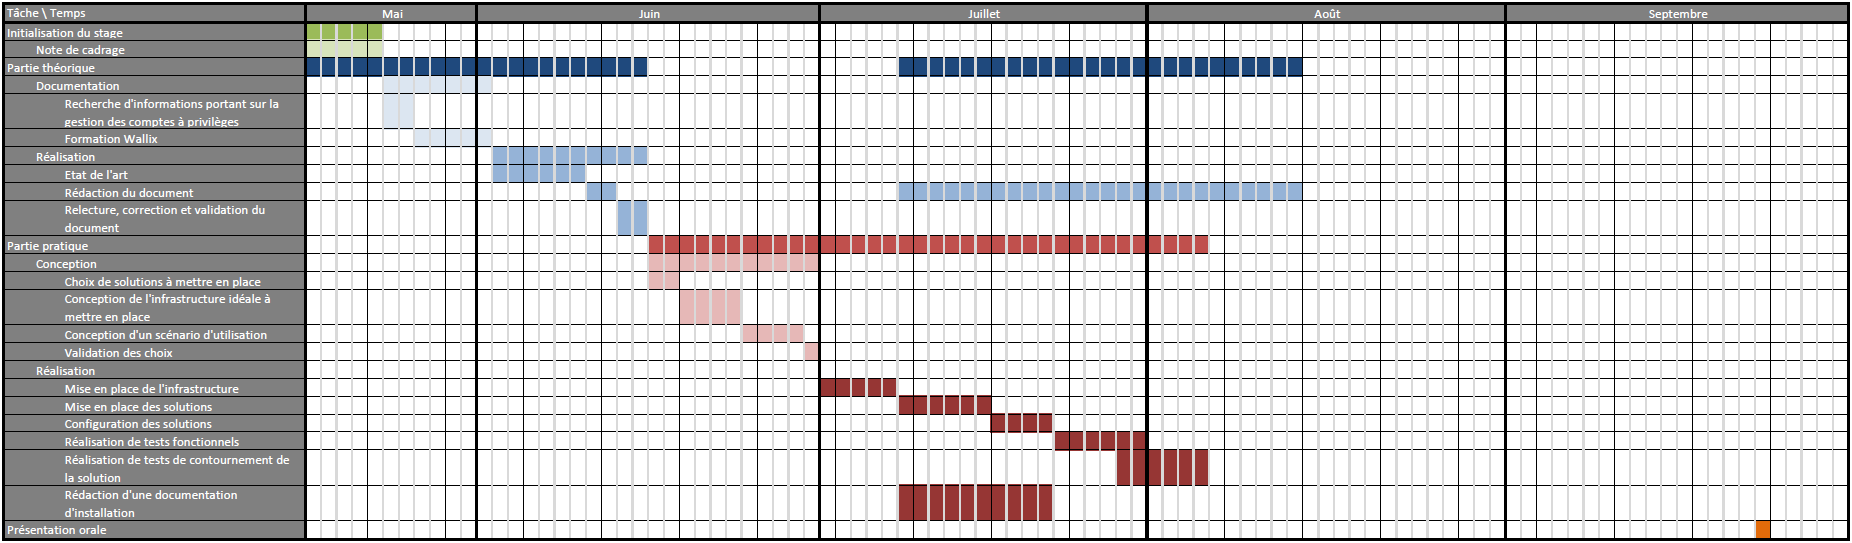
\includegraphics[width=\textwidth]{./images/calendrier_previsionnel.png}
    \caption{Calendrier prévisionnel}
\end{figure}

Bien sûr, le calendrier est une estimation et la réalité s'est avérée différente, ce point est abordé en section \ref{sec:resultats}. : la durée de recherche sur la gestion de comptes à privilèges et sur les différentes solutions a pris presque 2 fois plus de temps que prévu, tout comme le déploiement des solutions et le test de ces dernières. Cependant, le calendrier prévisionnel étant vu avec une large marge d'erreur, le stage tout de même pu être complété dans la durée impartie.

\subsection{Recherche}
\label{subsec:recherche}

La première étape a été la recherche d'informations sur le sujet. N'ayant pas de notions sur le sujet, j'ai d'abord commencé par me renseigner auprès des consultants de l'agence de Rennes, notamment mes tuteurs, Damien Seiler et Philippe Rolland, ainsi que le manager de l'agence, David Geffroy, ayant une base d'expertise dans le domaine. Grâce à ces premières lignes directrices fournis par ceux qui sont devenus mes collègues, j'ai pu orienter mes recherches internet vers la bonne direction, afin de trouver un maximum de résultats.

\subsubsection{Recherche du fonctionnement des solutions}
\label{par:fct_sol}
La meilleure façon de trouver des informations concernant le fonctionnement d'une solution de PAM s'est d'abord orientée vers la recherche d'informations génériques, comme des tutoriels ou des articles traitant du sujet. Cependant, j'ai fini par réaliser qu'il y avait très peu de ces ressources. La solution fut donc de directement s'orienter vers les solutions des éditeurs, et de tenter de comprendre leur fonctionnement, pour en tirer moi-même un fonctionnement général des solutions. Cette étape resta tout de même laborieuse, les éditeurs ne partageant pas énormément d'information quant à l'architecture ou le fonctionnement technique de leurs solutions, mais plutôt des caractéristiques de leur solution. Ceci ne m'empêcha pas de pouvoir trouver assez de solutions pour pouvoir en déduire une architecture assez claire, qui me donnait une vision d'ensemble du fonctionnement\footnote{Fonctionnement décrit dans un schéma en \textsc{Annexe}} d'une solution de PAM.\\
\textbf{INCLURE L'EXPLICATION DE FONCTIONNEMENT EN DÉTAIL ICI ?}

\subsubsection{Recherche des solutions existantes sur le marché}
\label{par:sol_market}
La recherche des solutions existantes sur le marché fut assez simple, compte tenu de la précédente recherche, s'appuyant sur ces solutions en question. Néanmoins, étant parti sur une base de 6 solutions trouvées pour réaliser un descriptif du fonctionnement général d'une solution de PAM, j'ai réussi à trouver plus du double de solutions par la suite, en navigant de lien en lien et en m'inscrivant à des newsletter m'envoyant des rapports tels que celui de l'éditeur \textsc{Forrester} écrit par Cser \cite{acs}.

\begin{figure}[!ht]
    \center
    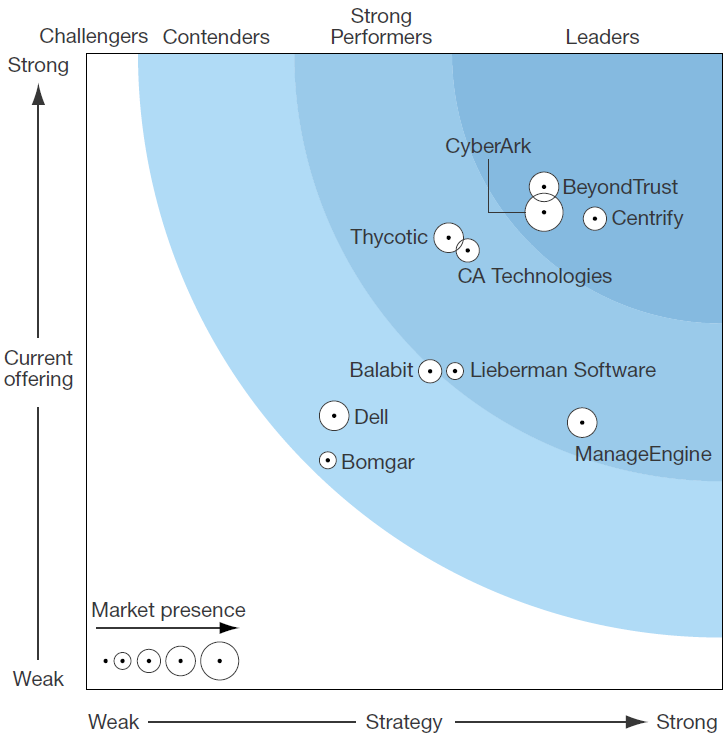
\includegraphics[width=0.7\textwidth]{./images/forrester_quadrant.png}
    \caption{Quadrant mettant en évidence les acteurs du marché de PAM selon le rapport offre/stratégie et l'indice de présence sur le marché}
\end{figure}

Nous avons ainsi pu nous retrouver avec une liste de solutions satisfaisante pour pouvoir commencer à faire un comparatif *réaliste* (terme à revoir). Nous avons alors orienté mes recherches vers les spécificités des solutions, en parcourant toute la documentation disponible, en participant à des vision-conférences avec les commerciaux et ingénieurs des maisons d'édition ou en contactant le support. Cette étape a été celle qui a pris le plus de temps dans la période de recherche, qui parfois s'est avérée infructueuse au vu du manque d'informations disponibles et de l'absence de réponse du support (ou plus précisément des réponses me redirigeant vers des documents en ligne ne contenant pas les réponses demandées). C'est par ailleurs une des étapes qui a complètement décalé le calendrier prévisionnel, prenant sur la marge prévue à cet effet.\\
Cette étape a conduit à éditer un tableau comparatif des solutions, dont nous pouvons trouver un aperçu à la \textsc{Figure }\ref{fig:tabcomp}. Ce tableau comparatif n'est pas disponible en annexe, à cause de sa taille impossible à imprimer, mais il reste tout de même disponible sur demande en format \emph{Microsoft Excel}.

\begin{figure}[!ht]
    \center
    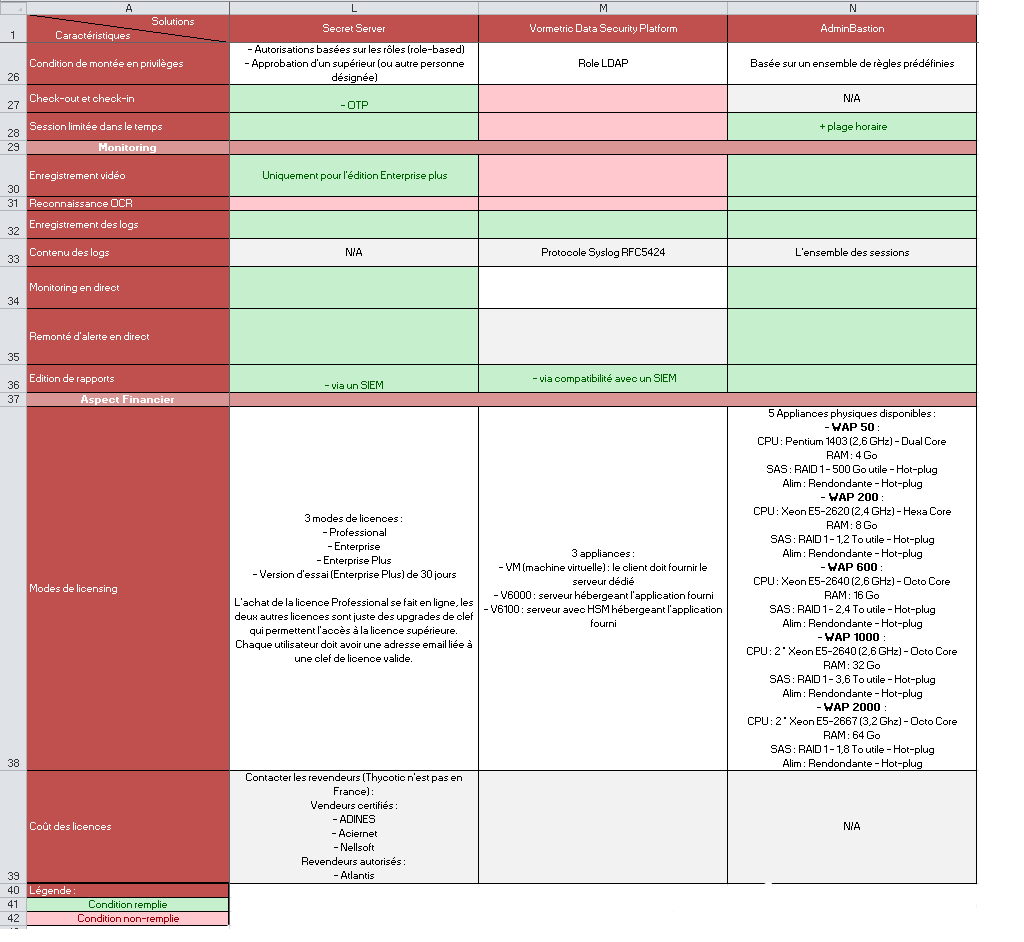
\includegraphics[width=\textwidth]{./images/tabcomp.png}
    \label{fig:tabcomp}
    \caption{Extrait du tableau comparatif de solutions édité au terme de la phase de recherche}
\end{figure}

\subsection{Proof of Concept}
\label{subec:poc}

La phase de conception d'environnement de test s'est déroulée en plusieurs étapes :
\begin{itemize}
	\item Conception architecture idéale
	\item Validation de l'architecture avec le tuteur, et remaniement de cette dernière pour s'adapter aux ressources matériels disponibles chez \textsc{Synetis}, ressources assez limitées car nous étions en saturation de ressources mémoire et processeur sur le serveur interne. Un nouveau serveur est arrivé en fin de stage, mais malheureusement quelques semaines trop tard
	\item Installation de l'infrastructure et déploiement des solutions à tester
\end{itemize}

\subsubsection{Architecture}
\label{par:archi}

L'architecture idéale sur laquelle les solutions devaient être intégrée nous semblait être celle qui se rapprochait le plus d'une situation réelle d'entreprise, comprenant des séparations logiques pour les différents corps de métier (

En effet, les ressources limitées ont réduit notre infrastructure de test au strict minimum, donc une machine de chaque type :
\begin{itemize}
	\item \textsc{MS Windows Server 2012 R2} : serveur de test de connexion RDP\footnote{Remote Desktop Protocol : contrôle à distance d'un serveur.}, de configuration des solutions de PAM (base de données \emph{MySQL} et \emph{SQL Server}), de mail (avec le logiciel \emph{hMailServer} \cite{hma} et contrôleur de domaine \emph{Active Directory}
	\item \textsc{MS Windows Server 2012} : serveur TSE\footnote{Terminal SErvice : permet d'utiliser le serveur pour faire tourner des applications utilisées en bureau distant.} permettant de tester une connexion sur une application distante (\emph{VMWare vSphere Client}\footnote{Programme Windows permettant de configurer un hôte de virtualisation et de faire tourner des machines virtuelles.} dans notre cas)
	\item \textsc{Linux Debian 8.4.0 Jessie} : serveur Linux permettant de tester une connexion SSH\footnote{Secure SHell : protocole de connexion à distance à une machine Linux/Unix.}
\end{itemize}

Cette architecture limitée nous a permis de tester et d'éprouver 2 des solutions choisies, tout en respectant les contraintes de ressources établies.\\
Bien plus que les solutions en elles-même, le déploiement de l'infrastructure de base a nécessité d'autres technologies, que l'ont peut lister en tâches suivantes :
\begin{itemize}
	\item Sur Microsoft Windows Server 2012 et 2012 R2 :
		\begin{arrowlist}
			\item Installation du rôle contrôleur de domaine\footnote{gestionnaire d'un domaine sous le système d'exploitation Windows.}
			\item Création et configuration d'un domaine, d'une forêt et de toutes ses dépendances assurant le bon fonctionnement de l'infrastructure
			\item Création d'utilisateurs de domaine\footnote{Utilisateurs créés dans un annuaire Active Directory, disponible pour toute machine du domaine.} avec les droits nécessaires et suffisant à leur fonctionnement, grâce aux groupes de sécurité Windows (consulter le livre de Minasi \emph{et al.} \cite{min} pour plus d'informations sur Active Directory et la sécurité de Windows Server 2012 R2)
			\item Création de comptes de service de domaine (MSA\footnote{Managed Service Account : compte Active Directory dédié aux service, le système gère lui-même les mots de passe.}) sous \emph{Powershell}\footnote{Interface en ligne de commande et langage de scripting dédié à Windows.}
			\item Installation de système de gestion de base de données relationnelle \emph{MySQL} et \emph{SqlServer} et création de bases de données pour les solutions de PAM
			\item Installation et configuration d'un serveur de mail local \emph{hMailServer} pour récupérer les mails envoyés par les solutions de PAM
			\item Installation du rôle TSE et configuration de ce dernier avec l'application \emph{VMWare vSphere Client}
		\end{arrowlist}
	\item Sur Debian 8.4.0 :
		\begin{arrowlist}
			\item Installation du serveur SSH
			\item Configuration réseau
		\end{arrowlist}
\end{itemize}

\subsubsection{Choix des solutions de PAM à tester}
\label{par:choixsol}

Nous avions fait, au terme de la phase de recherche, une sélection de 3 potentielles solutions à déployer sur nos environnements de test. Ce choix s'était fait en prenant en compte les données présentées dans le tableaux comparatif des solutions dont on a un aperçu dans la \textsc{Figure} \ref{fig:tabcomp}. Ces 3 solutions étaient :
\begin{itemize}
	\item \textsc{Wallix AdminBastion}
	\item \textsc{CyberArk Privileged Account Security Suite}
	\item \textsc{Thycotic SecretServer}
\end{itemize}

Nous étions déjà en contact avec \emph{Wallix}, car partenaires et mon tuteur était en train de passer une formation avec eux, pour la solution en question. Nous avons donc pu avoir facilement une installation de leur solution. En revanche, étant partenaire de \emph{Wallix}, \emph{CyberArk} a refusé de nous fournir une version d'évaluation tant que nous n'abandonnions pas notre partenariat, afin qu'il devienne notre partenaire exclusif. Ce choix de \emph{CyberArk} venant du fait que \emph{Wallix} est leur plus gros concurrent en France, car \emph{Wallix} est une entreprise Française et que beaucoup d'entreprises jouent le jeu de faire fonctionner une entreprise locale\footnote{Information fournie par le troisième éditeur, \emph{Thycotic} durant des échanges de mails.}. Nous avons donc déclineé la solution de \emph{CyberArk} et sommes entrés en contact avec \emph{Thycotic}, avec qui nous n'avons pas eu de soucis et qui nous ont offert un suivi remarquable (une communication omniprésente à toutes les étapes de test).

\subsubsection{Déploiement : Wallix AdminBastion}
\label{par:wallix}

La version d'essai de \emph{Wallix AdminBastion} se présente sous forme d'une machine virtuelle (fichier \texttt{vmdk}\footnote{VMWare Virtual Disk : format de disque virtuel créé par \emph{VMWare}}).\\
Cette machine virtuelle est un Debian 8 personnalisé par Wallix, avec leur propre configuration d'usine. Cette machine doit utiliser une base de données \emph{MySQL} externe afin de stocker ses données (logs et accréditations). Nous avons donc créé une base de données sur le serveur \emph{MySQL}
  \cleardoublepage
  \section{Résultats et discussion}
\label{sec:resultats}

Dans cette partie, nous allons discuter des résultats obtenus, pour déterminer s'il y a une solution plus à même de répondre aux besoins d'une entreprise avec laquelle \textsc{Synetis} pourrait envisager travailler.

\subsection{Des solutions se démarquant par des spécificités}
\label{subsec:soltaille}

Après avoir travaillé avec les deux différentes solutions (\emph{Wallix} et \emph{Thycotic}), il s'est clairement imposé que ces solutions apportent une approche similaire de la gestion des comptes à privilèges. Cette ressemblance d'utilisation a aussi été pointée lorsque je réalisais les PoC par l'étude de marché produit par l'entreprise de conseil Gartner\footnote{Gartner est une entreprise américaine de conseil et de recherche fondée en 1979. Elle vend des recherches et des analyses dans le domaine des technologies de l'information.} \cite{gar}. Les seuls gros points notables les différenciant sont la haute disponibilité qui n'est pas présente chez \emph{Thycotic}, la gestion des interactions d'application à application absente chez \emph{Wallix} et les formats de licences ne se recoupant que sur la disponibilité en mode \og cloud \fg{}.\\
Nous pouvons aussi noter une différence majeure entre ces deux solutions, au niveau des choix technologiques : \emph{Wallix} a choisi de développer sa solution sous Linux, tandis que \emph{Thycotic} s'appuie sur un système Windows Server. Ceci implique une facilité d'installation non-négligeable pour \emph{Wallix}, ne nécessitant pas de configuration préalable car l'ensemble du moteur du bastion est contenu dans la machine virtuelle (ou serveur physique, selon la licence choisie). Cette solution est complète, pour ainsi dire \og prête à l'emploi \fg{} car il ne reste que la configuration des ressources et utilisateurs à gérer. A l'opposé, \emph{Thycotic} fourni un exécutable à installer sur un serveur Windows, avec plusieurs solutions lourdes\footnote{Le serveur Windows d'une part, puis Microsoft SQL Server, Microsoft Internet Information Services et .NET Framework pour faire tourner l'interface de la solution.} à installer au préalable. Cette configuration n'a en l'occurrence pas fonctionné dans notre cas avec un serveur de test, il nous a fallu reprendre une installation \gls{stratch}.\\
Il faut aussi ajouter à cela que l'ensemble de la sécurité de \emph{Secret Server} s'appuie sur la sécurité du système d'exploitation Windows. Etant le plus touché par les attaques et donc le plus susceptible de connaître des failles de sécurité, comme l'ont démontré Sundar \textsc{et coll.}\cite{skk} sur une faiblesse de Windows Server 2012 R2 (soit la dernière version de Windows Server) face à une attaque de type DDoS (Syn flood\footnote{Bombardement de requête TCP SYN}).
%Expliquer pourquoi c'est de la merde Windows

\subsection{L'avenir dans le cloud}
\label{subsec:avenircloud}

Selon l'étude de Gartner\cite{gar}, les besoins de solution de \gls{pam} dans le cloud représentent seulement 3\% des parts de marché, pour, selon leur estimation, 30\% en 2019. Ces chiffres ne sont pas surprenants compte tenu de l'évolution des infrastructures décentralisées, comme le proposent les grands éditeurs comme Microsoft avec la suite \emph{365}, le géant du net Google avec son \emph{Google Enterprise}, Amazon avec l'ensemble de ses solutions qui vont du stockage de données (\emph{Amazon EC2}) au cluster de calcul (\emph{Amazon S3}).\\
Il est important de noter que cette gestion des comptes à privilèges dans le cloud représente un certain défi, sachant que ces infrastructures ne sont pas maintenues par les entreprises concernées (client final) mais par ces grands éditeurs. On peut alors se poser des questions sur la responsabilité des comptes à privilèges : relève-t-elle du client ou de l'éditeur ?

\subsection{Une synergie entre solution de PAM et une fédération d'identité}
\label{subsec:syner}

Un des leaders du marché des solutions de \gls{pam}, \emph{Centrify} (voir l'étude de marché menée par \textsc{Cser} \cite{acs} pour plus d'informations), propose un produit apportant une synergie entre la gestion des comptes à privilèges et la fédération d'identité\footnote{Gestion des accès et supervision des utilisateurs communs, par exemple la gestion des comptes des étudiants à l'université.}. En effet, il semble logique d'intégrer une solution de gestion des comptes à privilèges avec une solution de fédération d'identités, la gestion des utilisateurs en sera facilitée, et l’homogénéité du système offrira une assurance de qualité de service. Cependant, \emph{Centrify} est pour le moment le seul à proposer une telle solution, avec Microsoft et sa solution MIM (Microsoft Identity Manager) qui inclut l'extension PIM (Privileged Identity Manager) gérant les comptes à privilèges avec des groupes Active Directory de sécurité à usage limité dans le temps (\emph{shadow group}, voir l'article de \textsc{Microsoft Technet} \cite{mic} pour pus d'informations).

\subsection{CamStudio 2.7.4 : expérience personnelle d'attaque par escalade de privilèges}
\label{subsec:camstudio}

Le poste de travail qui m'a été fourni durant ce stage était un ordinateur de dépannage servant pour les nouveaux arrivants à \textsc{Synetis} Rennes. Au bout de quelques mois de stage, j'ai eu une notification douteuse me demandant de mettre à jour un logiciel (Yahoo! Search) qui n'étais pas installé sur le poste. Avec l'aide de plusieurs collègues, nous avons donc cherché à comprendre d'où venait cette notification, ce qui l'exécutait et quelles actions elle générait.\\
Nous avons commencé par suivre le processus avec le gestionnaire de tâches de Windows. Le processus était déclenché par un fichier présent dans le répertoire \texttt{AppData}, qui est le répertoire de stockages de données des applications s'exécutant sur Windows. Le fichier ayant lancé le processus (fichier avec une extension .dat) n'existait plus, mais il restait cependant un fichier de logs conséquent (plus de 1000 lignes de logs). Ce fichier nous a donné des informations sur les tentatives d'exécution de code sur la machine, en l'occurrence beaucoup d'ouvertures de shell, infructueuses avec le compte local. Un tel accès pourrait mener à une compromission complète du poste de travail, pouvant se traduire par un destruction du système, ou pire encore, un vol de données. Le vol de données serait le pire des scénario, si l'on tient compte que \textsc{Synetis} est un sous-traitant/intégrateur de solution de fédération d'identités pour des grands groupes tels que EDF ou encore des conseils régionaux, détenant ainsi les accès à l'administration de leur infrastructure.\\
Par la suite, nous avons trouvé comment était exécuté la fenêtre qui apparaissait : c'était une ancienne technologie, un fichier hta exécuté par un moteur de Windows. Ce moteur permet de convertir n'importe quel fichier binaire en page html dans une fenêtre embarquée. Nous avons réussi à trouver où menait le lien présent sur cette fenêtre : vers deux domaines qui ne répondaient pas lorsque l'on essayait de les joindre via un navigateur web. Ceci était sûrement dû à des paramètres traitant la requête sur le serveur n'acceptant que un certain type de requête, par exemple un \texttt{user-agent}\footnote{Dans une requête HTML, l'\texttt{user-agent} est le type de client lançant la requête, dans notre cas, notre navigateur web, par exemple Mozilla Firefox.} spécifique.\\
Après une recherche sur le net, nous avons trouvé un sujet ouvert sur le forum \emph{Reddit} discutant de ce malware, qui s'avère être présent dans une installation du logiciel CamStudio 2.7.4 compromis.\\
Finalement, la désinstallation de ce logiciel a empêché le malware de nuire. Toutefois, c'est une situation dans laquelle une solution de \gls{pam} aurait bloqué le problème à la source, en limitant l'installation d'un tel logiciel, si l'on considère que même l'installation de logiciel sur un poste est géré par les administrateurs de l'entreprise.

\subsection{Les bonnes pratiques à intégrer}
\label{subsec:pratiques}

Même avec une infrastructure sécurisée au plus proche de la perfection, les plus grosses failles restent l'humain. Il est donc important, lors d'un déploiement de solution de \gls{pam} de sensibiliser le personnel à certaines bonnes pratiques de sécurité incontournables. Ces pratiques sont détaillées dans une publication faite par le \textsc{NIST}\footnote{National Institute of Standards and Technology : institut national des standards et de la technologie des USA.} \cite{nist}.

\subsubsection{Renforcer l'authentification}
\label{par:auth}

Comme il a été vu en introduction, l'utilisation de mot de passe faible, devinable par ingénierie sociale\footnote{Deviner le mot de passe d'une personne en se renseignant sur ses habitudes, sa vie et ses relations sociales.}, d'algorithme de hachage faible, ou un faible chiffrement d'un mot de passe qui serait recouvrable par une \emph{rainbow table}\footnote{Table de correspondance de mots et de leur hash, disponible et utilisable en ligne.}.\\
Pour éviter de rencontrer des infiltrations par ces failles, il est important de mettre en place une politique de renforcement de l'authentification avec :
\begin{itemize}
	\item Une authentification forte : multi-facteur, au minimum double-facteur, par exemple l'utilisation du couple login/mot de passe et d'une validation avec envoi de SMS sur le téléphone personnel de l'employé. Plusieurs solutions déjà implémentés sont utilisables, comme par exemple \emph{Google Authenticator} ou le MFA de \emph{Microsoft}. Il est aussi possible de mettre en place un système PIV (Personnal Identity Verification, souvent une carte à puce à insérer dans un lecteur).
	\item Une augmentation des couches de sécurité dans le chiffrement des mots de passe : utilisation d'un algorithme de hachage fort comme le SHA-256 ou AES-256 doublé d'un salage (comme l'explique durant la conférence Blackhat US 2013 \textsc{Aumasson} \cite{jpa}) de ce hash avec une chaîne aléatoire.
	\item La mise en place d'une politique de mot de passe forte qui force l'utilisateur à utiliser un mot de passe d'une longueur minimale, avec un nombre minimal de caractères spéciaux, lettres minuscules et majuscules et chiffres. Il est même recommandé d'utiliser un passphrase, qui augmente la taille de la chaîne de caractères, en remplaçant les lettres par des chiffres et des symboles\footnote{Par exemple "4" pour "A", "\$" pour "s", etc.}.
\end{itemize}

\subsubsection{Minimiser les accès privilégiés}
\label{par:minipriv}

Le but de ce stage étant la gestion des comptes à privilèges, nous avons clairement pu comprendre que le meilleur moyen de limiter les compromissions de système était de limiter au maximum les accès privilégiés. La pratique est donc de commencer par :
\begin{itemize}
	\item Supprimer les accès des comptes à privilèges qui ne nécessitent plus ce type d'accès (par exemple l'administration de système, réseau ou base de données qui sont des tâches ponctuelles).
	\item Supprimer ou désactiver tous les comptes à privilèges qui ne sont plus nécessaires (y compris les comptes natifs du système).
	\item Supprimer l'excès de privilèges d'un compte en tenant compte du contexte de l'entreprise, plus que celui applicatif.
	\item Supprimer toutes les permissions inutiles des comptes à privilèges, notamment les commandes non-relative à l'utilisation de ces comptes.
	\item Réduire au minimum la durée d'une session privilégiée unique.
	\item Exiger une re-connexion lorsque cette dernière a expiré.
\end{itemize}


  \cleardoublepage
  \section*{Conclusion}
\addcontentsline{toc}{section}{Conclusion}

Pour conclure, avec \LaTeX{} on obtient un rendu impeccable mais il faut s'investir pour le prendre en main.

  \cleardoublepage
  \phantomsection\addcontentsline{toc}{section}{Références}
\begin{thebibliography}{ABC}	
    \bibitem[1]{rba} R.\textsc{Baloch} \emph{Ethical Hacking Penetration Testing Guide}, Auerbach Publications; 1 edition, 531 pages, 2014.
    \bibitem[2]{acs} Andreas \textsc{Cser} \emph{The Forrester Wave\texttrademark: Privileged Identity Management}, \textsc{Forrester$^{\mbox{\scriptsize{\textregistered}}}$}, Q3 2016.
    \bibitem[3]{hma} \textsc{hMailServer}. Page consultée le : 02/08/2016. \emph{Functionality - hMailServer - Free open source email server for Microsoft Windows}, Site web. \textsc{URL} : https://www.hmailserver.com/functionality
    \bibitem[4]{min} \textsc{Minasi}, \textsc{Mark}, et al. \emph{Mastering Windows Server 2012 R2}, John Wiley \& Sons, 2013.
    \bibitem[5]{jew} James E. \textsc{Weber}, Dennis \textsc{Guster}, Paul \textsc{Safonov} \& Mark B. \textsc{Schmidt}, \emph{Weak Password Security: An Empirical Study}, Information Security Journal: A Global Perspective, 17:1, 45-54, DOI:10.1080/10658980701824432, 2008.
\end{thebibliography}

  \cleardoublepage
  \section*{Annexe A}
\addcontentsline{toc}{section}{Annexe A}

\subsection{Fonctionnement détaillé des solutions de PAM}

Nous détaillerons dans cette annexe, le fonctionnement détaillé d'une solution de PAM. Afin d'illustrer les propos tenus, nous nous appuierons sur des schémas et digrammes de séquences.\\
Avant d'expliquer le fonctionnement d'une solution de PAM, nous allons voir comment les systèmes fonctionnent en temps normal.

\subsubsection{Sans solution de PAM}
\label{par:nopam}

Dans ce scénario, les utilisateurs finaux possèdent le mot de passe d'accès direct à la ressource protégée, comme on peut le voir sur la \textsc{Figure} \ref{fig:sans_PAM}.

\begin{figure}[!ht]
    \center
    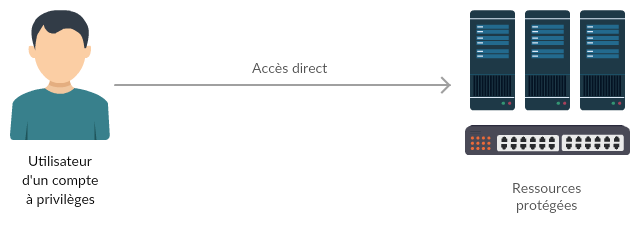
\includegraphics[width=\textwidth]{./images/Schema_ultra_light_sans_PAM.png}
    \caption{Connexion à une ressource protégée sans solution de PAM}
    \label{fig:sans_PAM}
\end{figure}

On remarque qu'ici, les utilisateurs accèdent directement aux ressources protégées avec des mots de passe dédiés à chaque service/application/matériel. Il est donc très fréquent car inévitable que des utilisateurs partagent le même mot de passe. De plus, n'ayant aucune fédération (pas de supervision, ni de traçage), l'utilisateur est apte à effacer ses traces, par exemple en vidant les logs des applications et de ses actions\footnote{Par exemple sous Debian 8, la commande \texttt{cat /dev/null > ~/.bash\_history \&\& history -c \&\& exit} supprime toute action effectuée sur la machine avec le compte courant.}. On ne peut donc pas savoir ce que l'utilisateur a fait, ni quel utilisateur a fait des actions sur la ressource cible.\\
Le diagramme de séquence en \textsc{Figure} \ref{fig:diagseq_sans_PAM} décrit en détail les action qui se déroulent lors d'une telle connexion. Il permet de ausi de mettre en évidence l'absence de contrôle des utilisateurs : aucun registre d'évènements ne prend en compte les actions des utilisateurs. Les utilisaterus se partageant le même mot de passe pour chaque ressource cible, le contrôle n'est ainsi plus mis sur les utilisateurs, mais sur les ressources cibles, ce qui est l'opposé de ce que nous cherchons à faire. La \testsc{Figure} \ref{fig:invcont} schématise cette inversion du contrôle. 

\begin{figure}[!ht]
    \center
    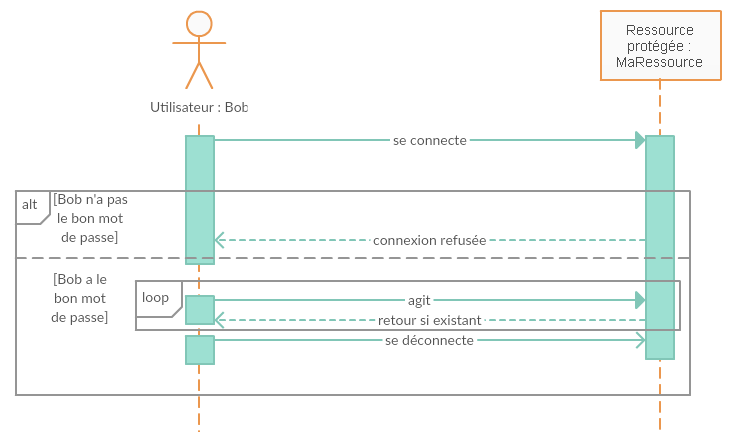
\includegraphics[width=\textwidth]{./images/Sequence_noPAM_use.png}
    \caption{Diagramme de séquence détaillant les actions effectuées lors d'une connexion à une ressource sans solution de PAM}
    \label{fig:diagseq_sans_PAM}
\end{figure}

\begin{figure}[!ht]
    \center
    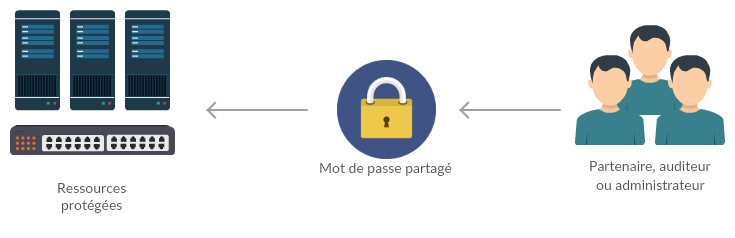
\includegraphics[width=\textwidth]{./images/ressource_centered.png}
    \caption{Schéma mettant en évidence l'inversion du contrôle de sécurité, mis sur les ressources plutôt que sur les utilisateurs}
    \label{fig:invcont}
\end{figure}

\subsubsection{Avec solution de PAM}
\label{par:withpam}

Dans ce scénario, une solution de PAM est en place. Ainsi les utilisateurs n'ont pas d'accès direct aux ressources cible. Toute l'architecture s'articule autour d'un composant central : le contrôleur d'accès appelé \textbf{bastion}. Tout accès à une ressource cible se fait via ce bastion. Cette architecture centralisée est schématisée dans la \textsc{Figure} \ref{fig:schempam}. Nous allons reprendre point par point un scénarion de connexion réussie à une ressource cible (en correspondance avec les étapes de la \textsc{Figure} \ref{fig:schempam}).

\begin{figure}[!ht]
    \center
    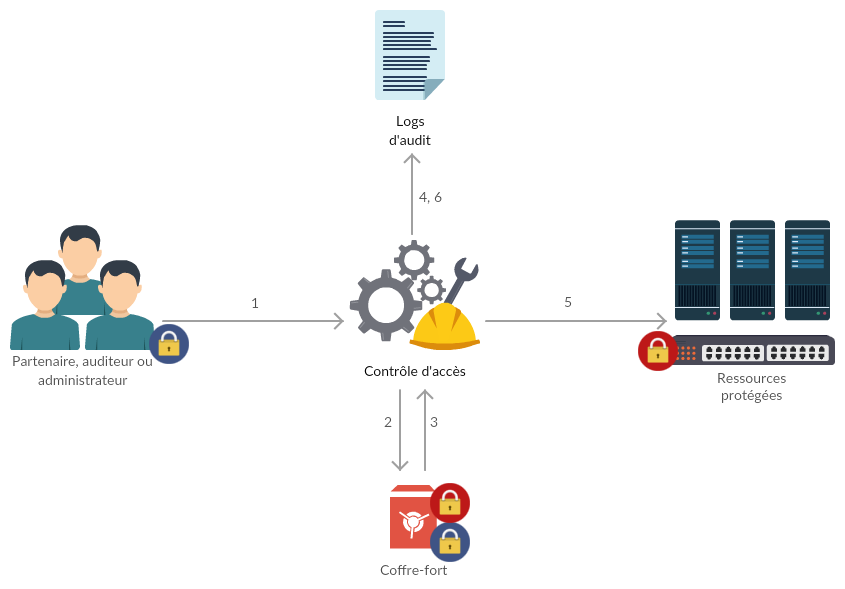
\includegraphics[width=\textwidth]{./images/Schema_PAM.png}
    \caption{Schéma décrivant l'architecture d'une solution de PAM intégrée dans une infrastructure}
    \label{fig:schempam}
\end{figure}

\begin{enumerate}
	\item L'utilisateur se connecte au bastion avec ses crédentiels
\end{enumerate}
  \cleardoublepage
  %\section*{Résumé} % Pas de numérotation

\paragraph{Résumé}
La gestion des comptes à privilèges est un domaine clef de la gestion d'accès et d'identité. Elle permet de suivre et journaliser les activités des comptes ayant des droits élevés comme \texttt{root} sur \textsc{Linux/UNIX} ou \texttt{Administrateur} sur \textsc{Windows}. Cette gestion permet ainsi de retrouver une erreur de configuration ayant entrainé une perturbation des services, de prévenir les intrusions par escalade de privilèges sur les système et de suivre d'éventuels prestataires de service dans un grand groupe (sous-traitance de la maintenance d'un service). Les solutions commerciales offrent différentes approches de la problématique des comptes à privilèges. Ce stage a donc fait l'objet d'une étude de ces différentes solutions, de leurs fonctionnalités et de leur fonctionnement. Cette étude a permis de faire ressortir 3 produits, \textsc{Wallix AdminBastion}, \textsc{CyberArk Privileged Access Security Solution} et \textsc{Thycotic Secret Server}, pour finalement en déployer 2 dans un environnement de test virtualisé. Cette mise en situation nous a permis d'aller plus en profondeur dans la compréhension du fonctionnement de la gestion des comptes à privilèges, des points traités et des points nécessitant des traitement supplémentaires à la diminution des risques des comptes à privilèges.

\subsubsection*{\center{Mots-clefs :}}

\center{sécurité, privilèges, compte, supervision, gestion}

%La gestion de comptes à privilèges (PAM\footnote{Privileged Access Management}) est une sous-section de la gestion d’identité et d’accès (IAM\footnote{Identity and Access Management}). L’IAM est un large champ de contrôle d’accès qui se veut critique dans le domaine des technologies de l’information.\\
%Il existe bien sûr une multitude de connexions spécifiques entre les utilisateurs et les dépendances technologiques. La PAM n’est que l’une d’entre elles.\\
%La PAM est apparue au début des années 2000 à cause de l’impossibilité des solutions d’IAM de contrôler, gérer et faire des rapports sur les accès aux serveurs, aux bases de données, aux équipements réseau et tout autre application critique au sein d’une organisation. Cette solution entraîne une gestion d’un petit nombre d’utilisateurs, mais d’un grand nombre de dépendances technologiques ayant une importance clef dans le fonctionnement des infrastructures.
  \cleardoublepage
  %\section*{Résumé} % Pas de numérotation

\paragraph{Abstract}
The management of privileged accounts is a key area of access and identity management. It can track and log activity of accounts with elevated privileges such as \texttt{root} on \textsc{Linux/UNIX} or \textsc{Windows} \texttt{Administrator}. This allows to recover a misconfiguration that caused a disruption of services, prevent intrusions by escalating privileges on the system, and monitor potential service providers in a large groups (outsourcing of maintenance service). Commercial solutions offer different approaches to the problem of privileged accounts. This internship has been the subject of a study of these different solutions, their functionalities and operation. This study allowed us to highlight three products: \textsc{Wallix AdminBastion}, \textsc{CyberArk Privileged Access Security Solution} and \textsc{Thycotic Secret Server}, to finally deploy in 2 proof of concept. This development has allowed us to go further in understanding the operation of the management of privileged accounts, treaties points and points requiring additional treatment to lower risk on privileges accounts.
\end{document}

